\chapter{Experiments}
\section{Authentication Scenario:}

In the following Java example the method createDBAccess is used to create a DBAccess object for a database management application.

\begin{lstlisting}
public DBAccess createAccount(String userName, String userType,
 String userPassword) {

		DBAccess access = new DBAccess();
		access.setUserName(userName);
		access.setUserType(userType);
		access.setUserPassword(userPassword);	
				
		return access;
}

\end{lstlisting}

However, there is no authentication mechanism to ensure that the user creating this database user account object has the authority to create new user access. Some authentication mechanisms should be used to verify that the user has the authority to create database access objects.
The following Java code includes a boolean variable and method for authenticating a user. If the user has not been authenticated then the createAccount will not create the database access object.

\begin{lstlisting}

private boolean isUserAuthentic = false;

// authenticate user,
// if user is authenticated then set variable to true
// otherwise set variable to false
public boolean authenticateUser(String username, String password) {
...
}

public DBAccess createAccount(String userName, String userType,
String userPassword) {
			DBAccess access = null;
			
			if (isUserAuthentic) {
			access.setUserName(userName);
			access.setUserType(userType);
			access.setUserPassword(userPassword);
		}
	return access;
}
\end{lstlisting}

Now let's model this kind of scenario in UML statechart considering that for C/C++ application.Figure \ref{authentication_scenario}  represents an authentication scenario. In this scenario a user A wants to access a database. At first he/she has to provide his/her user id, password, account number. Then he/she sends request to access database. The database administrator creates a user using his/her id,name and password based on their policy. According to the policy user can either view or access the database or not. If database server doesn't have some secured policy like validation,encryption, decryption or authentication methodology then hacker may easily break the application and receives the confidential information or data from the database server. In Figure \ref{authentication_scenario} depicts a highly secured variable \enquote{char *a} which is initially annotated as H. It passes through a function named authentication. This authentication function is represented as a state in the statechart as like \enquote{void declassification(char *a)}. This function makes the high secured variable as low by following the policy language. After passing these function the variable \enquote{char *a} is annotated with L and authenticated. Now it can be passed to other system or release information to the authenticated user.

\begin{figure}[htbp]
	\centering
	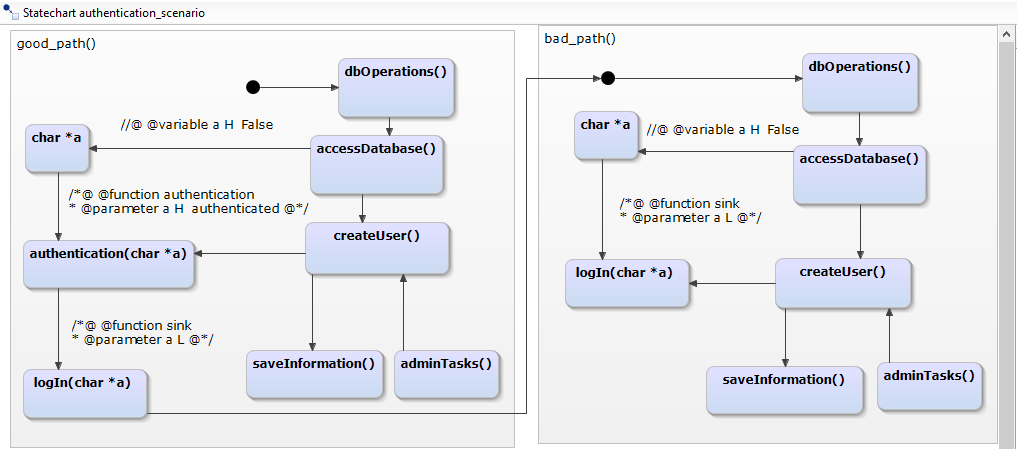
\includegraphics{styles/authentication_scenario.png}
	\label{authentication_scenario}
	\caption{Authentication Scenario}
\end{figure}

\section{Declassification Scenario:}
 Noninterference is typically
 too strong a property, most programs use some form of declassification to selectively leak high security information, e.g. when performing a password check or data encryption. Unfortunately, such  a declassification is often expressed as an operation within a given  program, rather than as part of a global policy, making reasoning about the security implications of a policy more difficult. For application programmers need to prevent a range
 of problems, from SQL injection and cross-site scripting, to inadvertent password disclosure and missing access control checks.Adding declassification function is one of the possibility for an application to detect information flow vulnerabilities. It requires few changes to the existing application code and an assertion of functions such as declassification, sanitization and authentication can reuse existing code and data structures. \\
 
 For the declassification scenario, a user A wants to access his bank account. Every bank has their own policy to their customer who can access their account information. After giving the password, account number, user name user A send his request to the bank server to view the account information. The bank server has his own policy according to their requirements. Through that policy bank server verifies the user A may be by following the basic declassification goals according to four axes like what information is released,
 who releases information, where in the system information is released and when information can be released.  \\
 
 Figure \ref{declassification_scenario}  represents a declassification scenario. In this scenario a user A wants to access his bank account. At first he/she has to provide his/her user id, password, account number. Then he/she sends request to access his/her account. The bank server has their own policy who can access the account details. According to the policy user can either view his account details or not. If bank server doesn't have some secured policy like encryption, decryption or declassification methodology then hacker may easily break the application and receives the confidential information or data. In Figure \ref{declassification_scenario} depicts a highly secured variable \enquote{char *a} which is initially annotated as H. It passes through a function named declassification. This declassification function is represented as a state in the statechart as like \enquote{void declassification(char *a)}. This function makes the high secured variable as low by following the policy language. After passing these function the variable \enquote{char *a} is annotated with L and declassified. Now it can be passed to other function or release information to the verified user.\\
 
 After finishing the modeling of declassification scenario then through the C code generator C code files are generated which consist two files(.c and .h file). Inside those files annotations are exist. Then through static analysis engine named \enquote{smtcodan} analyze the code and detect the information flow vulnerabilities if they exist inside the generated files.
 
\begin{figure}[htbp]
	\centering
	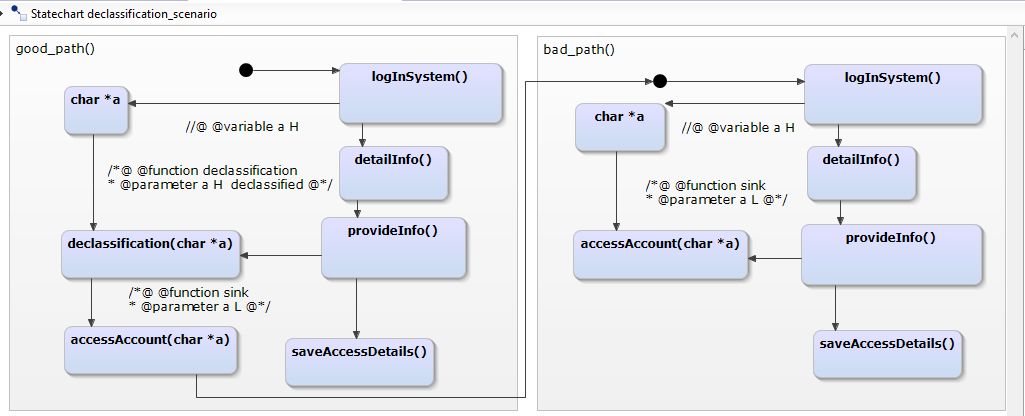
\includegraphics{styles/declassification_scenario.png}
	\label{declassification_scenario}
	\caption{Declassification Scenario}
\end{figure}


\section{Sanitization Scenario:}
Web applications are often implemented by developers with limited security skills.As a result, they
contain vulnerabilities. Most of these vulnerabilities stem
from the lack of input validation. That is, web applications
use malicious input as part of a sensitive operation, without having properly checked or sanitized the input values
prior to their use.
In the past research on vulnerability analysis has mostly focused on identifying cases in which a web application directly uses external input in critical operations. However,
little research has been performed to analyze the correctness of the sanitization process. Secured web application helps to prevent the bad guys from gaining unauthorized access to your application/site's data. It helps you keep your data's integrity and ensures availability as needed. Sql injection and XSS attacks are common attacks now-a-days. to prevent this kind of attacks need to use sanitization methods and validate user input properly.\\
This example code intends to take the name of a user and list the contents of that user's home directory. It is subject to the first variant of OS command injection.Example language is in PHP.

\begin{lstlisting}
	$userName = $_POST["user"];
	$command = 'ls -l /home/' . $userName;
	system($command);
\end{lstlisting} 

The userName variable is not checked for malicious input. An attacker could set the userName variable to an arbitrary OS command such as:
\begin{lstlisting}
;rm -rf /
\end{lstlisting}
Then that would produce a result like this-
\begin{lstlisting}
ls -l /home/;rm -rf /
\end{lstlisting}
Since the semi-colon is a command separator in Unix, the OS would first execute the ls command, then the rm command, deleting the entire file system.\\

The previous example was given for PHP language. In C language here it has been selected that user \enquote{A} wants to access some file from server pc. So, he needs to give the file name. If he wants to access some exe file then bug should be triggered or if he inserts some OS command injection type of statement then bug should be triggered. That's why the user input should pass through a sanitization method to sanitize the input parameter.\\

 Figure \ref{sanitization_scenario} depicts a sanitization scenario. In this scenario a user A wants to access file from a server. At first he/she has to provide file name. Then he/she sends request to access his/her desire file. The server has their policy who can access the file. According to the policy if the server has proper sanitization methods then by sanitizing the user input server either allow or disallow the user to access the file. If bank server doesn't have some secured policy like encryption, decryption or sanitization methodology then hacker may easily break the application and receives the confidential information or data, even execute the .exe files or may do some OS command injection. In Figure \ref{sanitization_scenario} shows a highly secured variable \enquote{char *a} which is initially annotated as H. It passes through a function named sanitization which also represented as a state named \enquote{void sanitization(char *a)}. This function makes the high secured variable as low by following the policy language. After passing these function the variable \enquote{char *a} is annotated with L and sanitized. Now it can be passed to other function or release information from the system.

\begin{figure}[htbp]
	\centering
	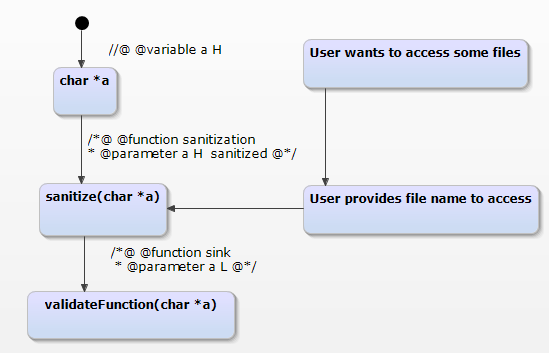
\includegraphics{styles/sanitization_scenario.png}
	\label{sanitization_scenario}
	\caption{Sanitization Scenario}
\end{figure}